\documentclass{beamer}
\usepackage[utf8]{inputenc}
\usepackage{amsmath}
\usepackage{mathtools}
\DeclareMathOperator*{\argmax}{argmax} % thin space, limits underneath in displays
\mode<presentation>{
\usetheme{Madrid}
\usecolortheme{TOSU}
}

\makeatletter
\newenvironment{myitemize}{%
   \setlength{\topsep}{0pt}
   \setlength{\partopsep}{0pt}
   \renewcommand*{\@listi}{\leftmargin\leftmargini \parsep\z@ \topsep\z@ \itemsep\z@}
   \let\@listI\@listi
   \itemize
}{\enditemize}

% Load biblatex package and .bib document
\usepackage{natbib}
\bibliographystyle{unsrtnat}

\AtBeginSection[]{
  \begin{frame}
  \vfill
  \centering
  \begin{beamercolorbox}[sep=8pt,center,shadow=true,rounded=true]{title}
    \usebeamerfont{title}\insertsectionhead\par%
  \end{beamercolorbox}
  \vfill
  \end{frame}
}

%Information to be included in the title page:
\title{News Article Classification}
\subtitle{(Multi-Label Learning: ML-KNN \& BP-MLL)}
\author[STAT 6500]{Lauren Contard, Archit Datar, Yue Li, Bobby Lumpkin, Haihang Wu}
\institute[OSU] % Your institution as it will appear on the bottom of every slide, may be shorthand to save space
{
The Ohio State University \\ % Your institution for the title page
\medskip
STAT 6500 % Your email address
}
\date{}



\begin{document}

\frame{\titlepage}

\begin{frame}
\frametitle{Overview} % Table of contents slide, comment this block out to remove it
\tableofcontents % Throughout your presentation, if you choose to use \section{} and \subsection{} commands, these will automatically be printed on this slide as an overview of your presentation
\end{frame}

\section{Introduction and Problem Statement}

\subsection{Introduction and Description of Datasets}

\begin{frame}[t]{Introduction}
    \small
    \begin{itemize}
        \item 
        People in the U.S. have shown polarized attitudes and behaviors in response to COVID-19.
        
        \item
        What could be some of the drivers? We aim to explore whether and how mainstream news media in the U.S. play a role in the polarization of the public's attitudes and behaviors.
    \end{itemize}
    
    \vskip
    \begin{figure}[htp]
        \centering
        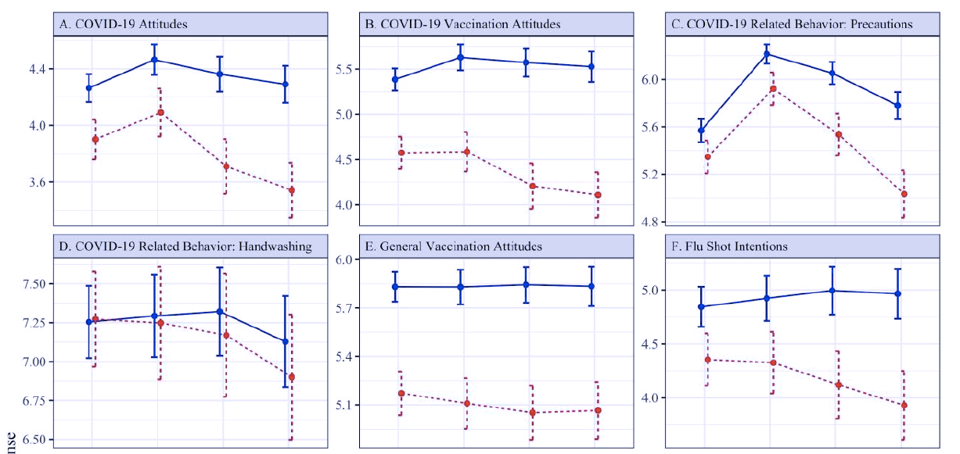
\includegraphics[width = 10cm]{Images/covid_polarization.png}
    \end{figure}
    
\end{frame}

\begin{frame}[t]{Description of Datasets}
    \small
    \begin{itemize}
        \item 
        We analyzed news content about elite communication from 10 news media, including newspapers (e.g., New York Times) and cable network news (e.g., ABC news).
        
        \item
        We got the list of news articles from the GDELT database and used the Python package "Scrapy" to get the full text.
        
        \item
        We have 8588 news articles in total and randomly selected 290 paragraphs of them to label. 
        
        \item
        We manually labeled our paragraphs into 15 categories. One paragraph usually has multiple labels.  
        
    \end{itemize}
    
\end{frame}

\begin{frame}[t]{Two Examples from the Dataset}
    \scriptsize
    "Meanwhile, Bottoms has repeatedly urged residents to stay home. On Friday, she tweeted coronavirus fatality statistics for the state: 'The numbers speak for themselves. PLEASE STAY HOME.'" (From USAtoday, 04/25/2020)
    \begin{itemize}
        \item 
        Threats/impacts
        \item
        Responses/actions
        \item
        Severity
        \item
        Self-efficacy
        \item
        Public Health
        \item
        Negative
    \end{itemize}
    "You know, I wonder, I think there's been a lot of self-congratulations every day that we see in those briefings, frankly, about the testing in the United States, and we're doing so well, we're doing now more than South Korea did." (From abcnews, 03/29/2020)
    \begin{itemize}
        \item 
        Responses/actions
        \item
        External-efficacy
        \item
        Public health
        \item
        Political evaluation
        \item
        Negative
    \end{itemize}
    
\end{frame}

\subsection{Problem Statement}

\begin{frame}[t]{Problem Statement}
    \small
    \begin{itemize}
        \item 
        We have a multi-label classification problem. We adapted two learning algorithms: k-NN and Neural Networks to handle multi-label data directly.
        
        \textbf{RQ1}: Which learning algorithm performs better in the multi-label classification problem: k-NN or neural networks?? 
        
        \item
        Our data has high dimensions.
        
        \textbf{RQ2}: How can we effectively implement linear and non-linear dimensions reduction in the multi-label classification problem?
        
        \item
        The sequence of features need to be considered in the classification.
        
        \textbf{RQ3}: Which type of the features perform better in the multi-label classification problem: with or without considering the order of words?
        
    \end{itemize}

    
\end{frame}

\section{KNN Based Approaches}

\subsection{Binary Relevance}

\begin{frame}[t]{Binary Relevance (A Naive Approach)}
    \small
    \begin{itemize}
        \only<1->{
        \item 
        An intuitive approach to deal with the multilabel paradigm.}
        
        \only<2->{
        \item
        Works by decomposing the multi-label learning task into a number of independent binary learning tasks (one per class label).}
    \end{itemize}
    
    \vskip-1.15em
    \only<3->{
    \begin{figure}[htp]
        \centering
        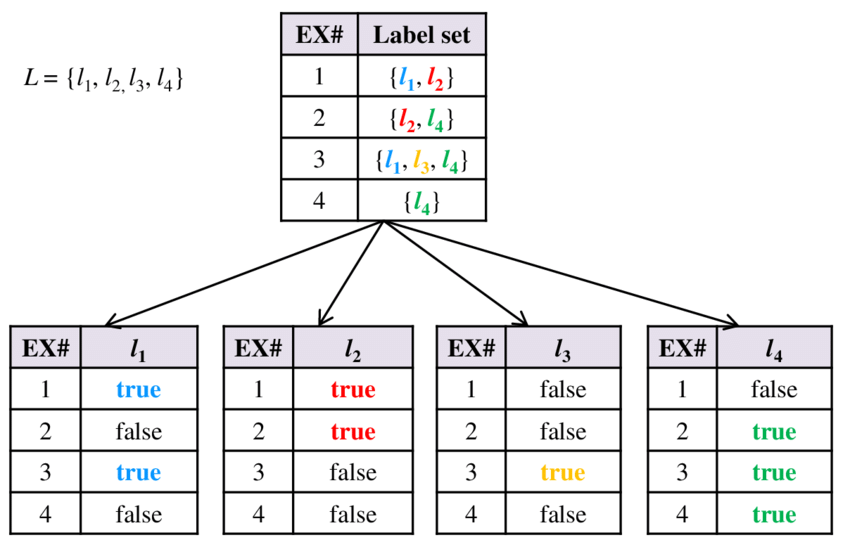
\includegraphics[width = 6cm]{Images/Binary-relevance-problem-transformation-method.png}
    \end{figure}}
    
    \vskip-1.25em
    \begin{itemize}
        \only<4->{
        \item[\rightarrow] 
        Often criticized in the literature because of its label independence assumption.}
        
        \only<5->{
        \item[\rightarrow]
        We implement a KNN based binary relevance model and compare with a more novel adaptation: the ML-KNN model.}
    \end{itemize}
    
\end{frame}

\subsection{ML-KNN Algorithm}
\begin{frame}[t]{ML-KNN Algorithm: Overall Approach}
\small
\textbf{Overall Approach:}
This ML-KNN algorithm takes a parametric, Bayesian approach towards estimating the Bayes Optimal Classifier. As with the single-label algorithm, it does this using the K nearest neighbors of an instance. Namely...

\begin{itemize}
	
		\item 
		Given a test instance, $t$, $\vec{Y}_t$ is determined using the MAP estimate:
	
	
		\begin{align*}
		\vec{y}_t(\ell) &= \argmax_{b \in \{0, 1\}} \mathbb{P}\left(\textrm{H}_b^\ell | E_{\vec{C}_t(\ell)}^\ell\right), \textrm{\hspace{0.3cm}}\ell \in \mathcal{Y} \\
		&= \argmax_{b \in \{0,1\}} \frac{\mathbb{P}\left(\textrm{H}_b^\ell\right) \cdot \mathbb{P}\left(E_{\vec{C}_{t(\ell)}}^\ell | \textrm{H}_b^\ell\right)}{\mathbb{P}\left(E_{\vec{C}_t(\ell)}^\ell \right)} \\
		&= \argmax_{b \in \{0, 1\}}\mathbb{P}\left(\textrm{H}_b^\ell\right) \cdot \mathbb{P}\left(E_{\vec{C}_{t(\ell)}}^\ell | \textrm{H}_b^\ell\right)
		\end{align*}
	
	
		\item
		Where we take a Bayesian approach towards estimating the prior probabilities, $\mathbb{P}\left(\textrm{H}_b^\ell\right)$, and conditional probabilities, $\mathbb{P}\left(E_{\vec{C}_{t(\ell)}}^\ell | \textrm{H}_b^\ell\right)$.
	\normalsize
\end{itemize}
\end{frame}


\begin{frame}[t]
\frametitle{ML-KNN Algorithm: Reasons for dimension reduction}
\begin{center}
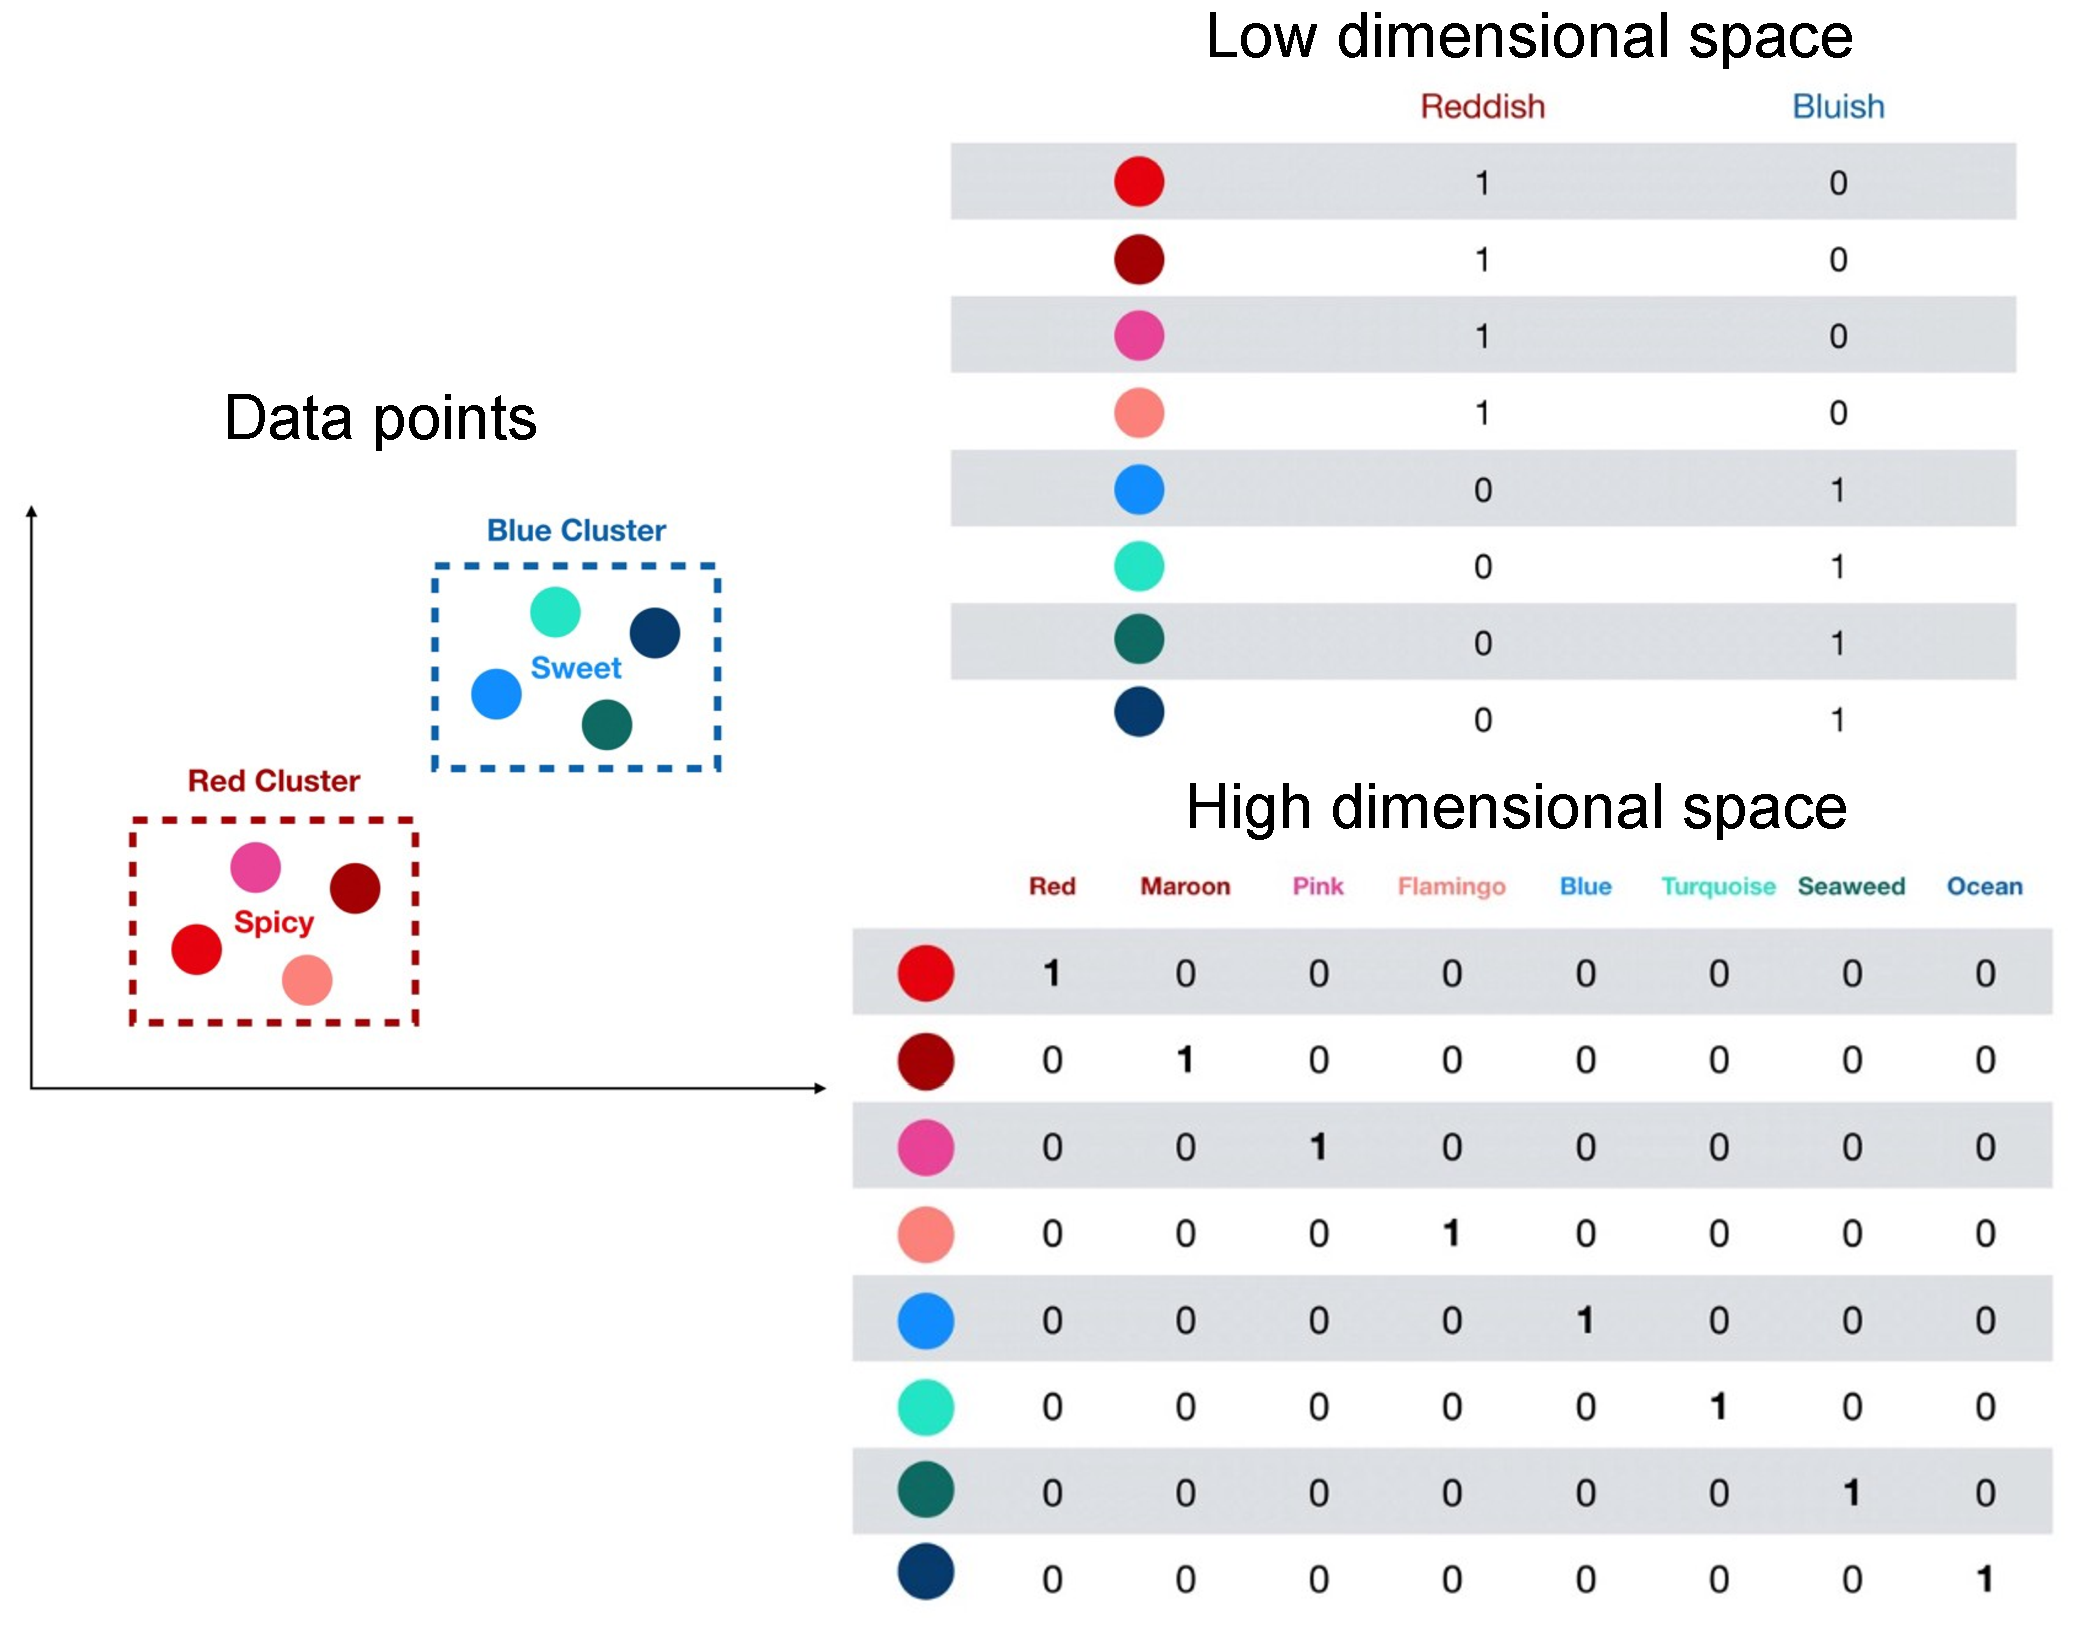
\includegraphics[width=0.7\textheight]{Images/DimRed.pdf}
\end{center}
Having a high dimensional feature space causes Euclidian distances between points to be fairly similar as the distance vector components are partitioned across many dimensions. 

%%\footnote{\cite{yiu}}
%%Archit's comments: How exactly do we cite so that the citation appears on the slide? 

\end{frame}

\begin{frame}[t]{Nonlinear Dimension Reduction (ANN Autoencoder)}
    \begin{itemize}
        \only<2->{
        \item 
        PCA allows only for reductions in dimension due to linear representations.}
        
        \only<3->{
        \item
        Autoencoders can learn data projections with suitable dimensionality and sparsity limitations that allow for nonlinear representations, as well.}
    \end{itemize}
    
    \vspace{-0.3cm}
    \begin{columns}[T]
        \column{0.5\textwidth}
        \begin{itemize}
            \vspace{0.5cm}
            
            \only<4->{
            \item[\rightarrow]
            Train a feed forward neural network with a "bottleneck layer" to perform the identity mapping.}
            
            \vspace{0.25cm}
            \only<5->{
            \item[\rightarrow]
            Use bottleneck layer values as encodings of the data.}
        \end{itemize}
        
        \column{0.5\textwidth}
        \only<4->{
        \begin{figure}[htp]
            \centering
            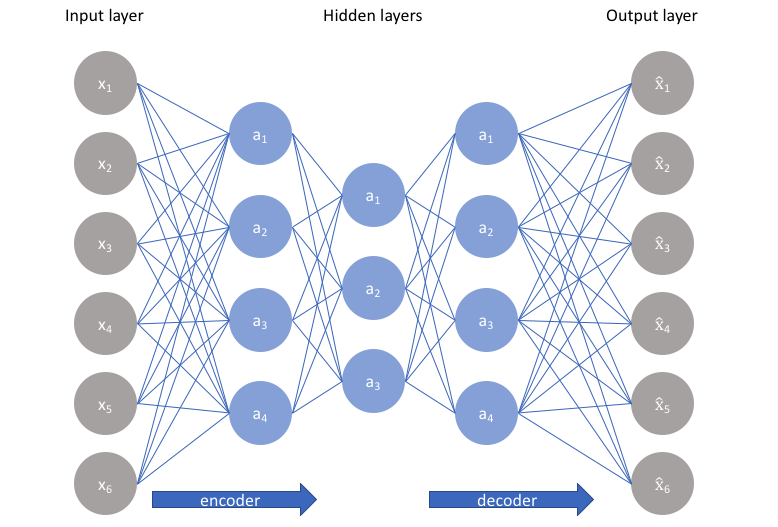
\includegraphics[width = 6cm]{Images/autoencoder_diagram.png}
        \end{figure}}
    \end{columns}
\end{frame}

\begin{frame}[t]{Threshold Function Learning}
    Perfect classification, using a constant threshold requires two conditions:
    \vspace{0.25cm}
    \begin{enumerate}
        \item 
        Predicted logit values for "true" labels be separated from predicted logit values for "false" labels.
        
        \item
        This separation be around some constant value (usually either $0.5$ or $0$)
    \end{enumerate}
    
    \vspace{0.15cm}
    Learning a threshold function aims to relax the second condition.
    
    \begin{itemize}
        \item[\rightarrow] 
        Namely, we fit a linear regression model to learn threshold values from the logit outputs of our models.
    \end{itemize}
\end{frame}

\subsection{Results}

\section{Neural Network Based Approaches}

\begin{frame}[t]{A Brief History}
    \scriptsize
    \begin{itemize}
        \onslide<2->{
        \item 
        Inspired by biological nervous systems, neural networks date back to the first half of the 20th century with works such as those by McCulloch and Pitts, which could model simple logical operations.}
            
    \end{itemize}
        
    \begin{columns}[T]
    \column{0.5\textwidth}
    \onslide<2->{
    \begin{figure}[htp]
        \centering
        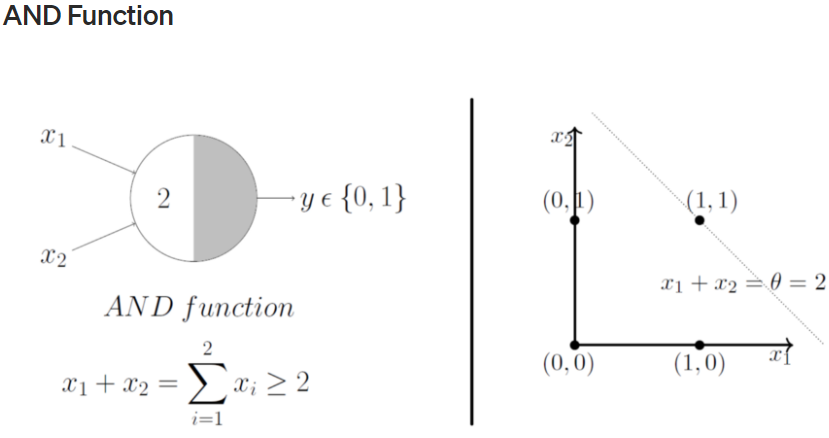
\includegraphics[width = 5cm]{Images/McCullochPitts_and_gate.PNG}
    \end{figure}}
    
    \column{0.5\textwidth}
    \onslide<2->{
    \begin{figure}[htp]
        \centering
        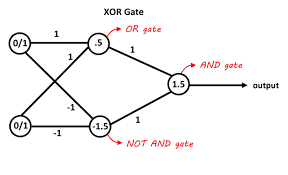
\includegraphics[width = 5cm]{Images/Multi_layer_McCullochPitts_XOR.png}
    \end{figure}}
    \end{columns}
    
    \onslide<2->{
    \begin{figure}[htp]
        \centering
        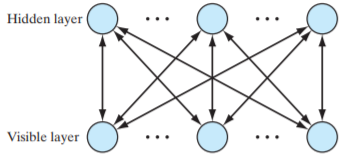
\includegraphics[width = 5cm]{Images/restricted_Boltzmann_machine_diagram.PNG}
    \end{figure}}
    
\end{frame}

\subsection{Architectures: Feed Forward \& Recurrent Networks}

\begin{frame}[t]{Network Architectures (Feed Forward vs Recurrent)}
    \small
    \vskip-2.5em
    \begin{columns}[t]
        \begin{column}{0.5\textwidth}
            \begin{center}
                \textbf{\underline{Feed Forward Networks}}
            \end{center}
            \begin{myitemize}
                \item 
                Neurons in the first layer represent components of the input vectors.
                
                \item
                The output of the neuron in the next layer is determined by applying a non-linear ``activation function" to a linear combination of the input components, plus a bias.
            \end{myitemize}
            
            \begin{figure}[htp]
                \centering
                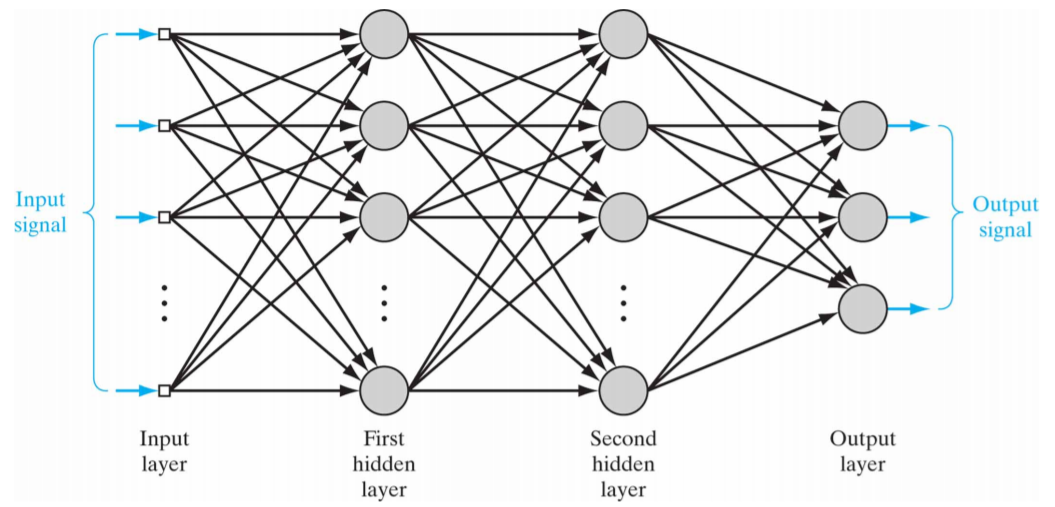
\includegraphics[width = 6cm]{Images/multilayer_network_Haykin.PNG}
            \end{figure}
        \end{column}
          
        \begin{column}{0.5\textwidth}
            \begin{center}
                \textbf{\underline{Recurrent Neural Networks (RNNs)}}
            \end{center}
            \begin{myitemize}
                \item 
                RNNs are a popular adaptation for NLP problems.
                
                \item
                They utilize hidden unit connections with shared weights.
                
                \item
                Unfolding an RNN let's us visualize it like a feed forward network (see below).
            \end{myitemize}
            
            \vskip-1em
            \begin{figure}[htp]
                \centering
                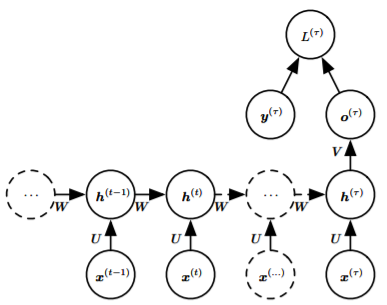
\includegraphics[width = 4cm]{Images/RNN_unfolded_goodfellow.PNG}
            \end{figure}
        \end{column}
    \end{columns}
\end{frame}

\subsection{Loss Functions: Cross Entropy vs BPMLL}

\begin{frame}[t]{Naive vs Novel Approaches (Cross Entropy vs BPMLL)}
    \begin{itemize}
        \item 
        By "naive" we refer to multilabel networks that utilize a cross entropy loss for training.
        
        \item
        By comparison, Zhang and Zhou \autocite{bpmll} proposed a novel loss, that emphasizes pairwise ranking accuracy.
        
        $$
            E = \sum_{i = 1}^m E_i = \sum_{i = 1}^m \frac{1}{|Y_i| |\overline{Y}_i|} \sum_{(k,l) \in Y_i \times \overline{Y}_i} \exp(-(c_k^i - c_l^i))
        $$
        so that the $i^{th}$ error term is severely penalized if $c_k^i$ is much smaller than $c_l^i$.
    \end{itemize}
\end{frame}

\subsection{Results}

\begin{frame}[t]
\frametitle{Artificial Neural Network Results: Full Dataset}
\begin{center}

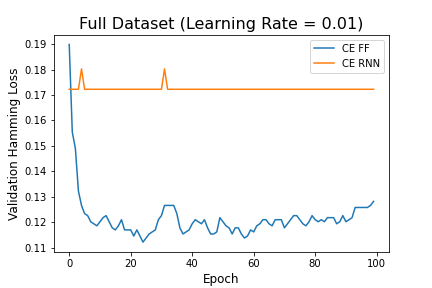
\includegraphics[width=0.32\textwidth,height=3cm]{Images/Full_Dataset_Learning_Rate_01.png}
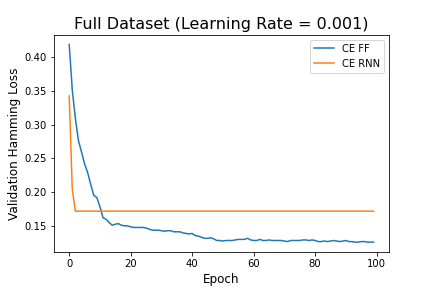
\includegraphics[width=0.32\textwidth,height=3cm]{Images/Full_Dataset_Learning_Rate_001.png}
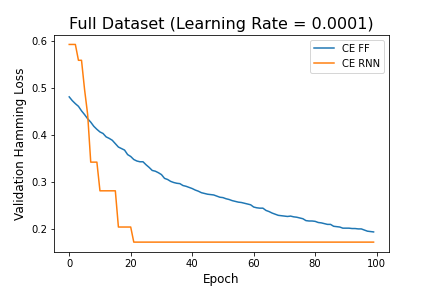
\includegraphics[width=0.32\textwidth,height=3cm]{Images/Full_Dataset_Learning_Rate_0001.png}        
\end{center}

\begin{center}

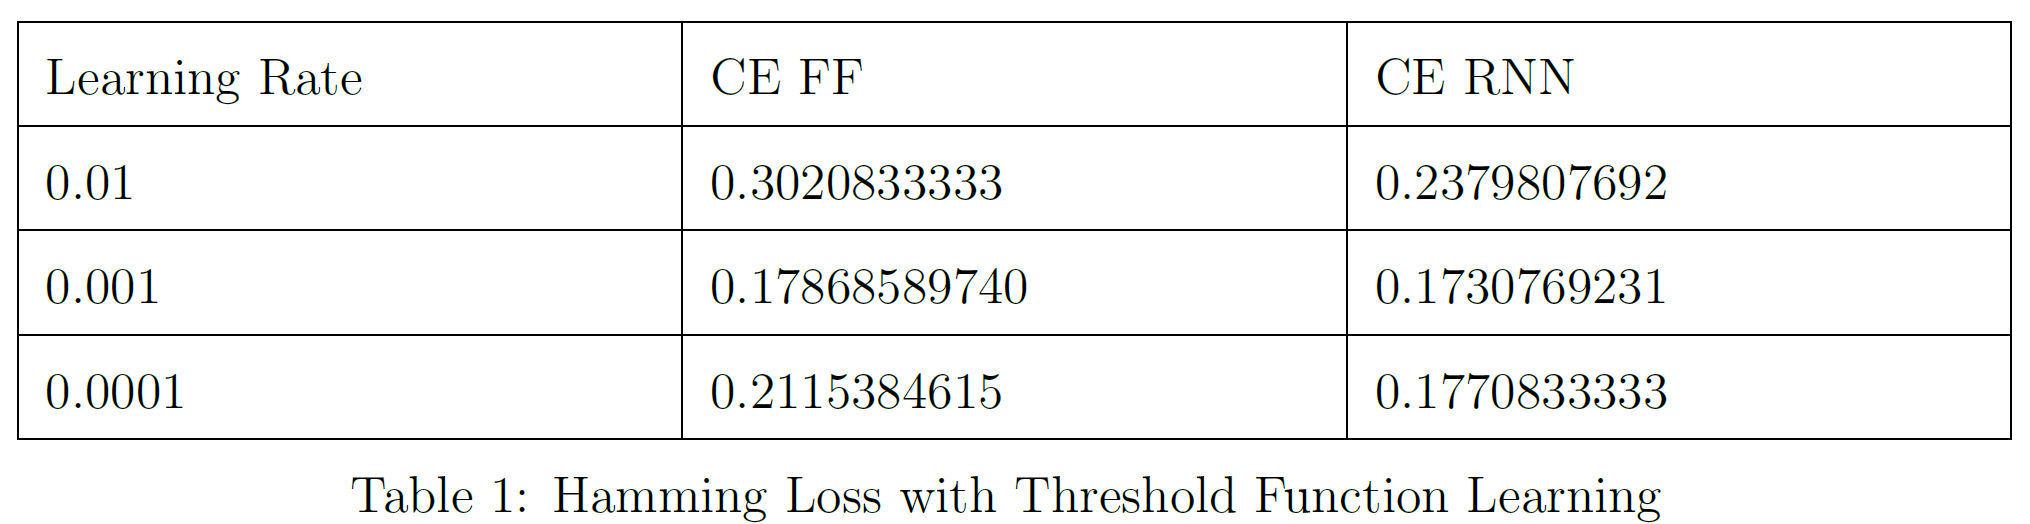
\includegraphics[width=1\textwidth,height=3cm]{Images/Threshold learning for full dataset.png}
\end{center}

CE FF outperform CE RNN in constant threshold but underperform in learned threshold; The effect of learning rate. 
\end{frame}

\begin{frame}[t]
\frametitle{Artificial Neural Network Results: Reduced Dataset}
\begin{center}

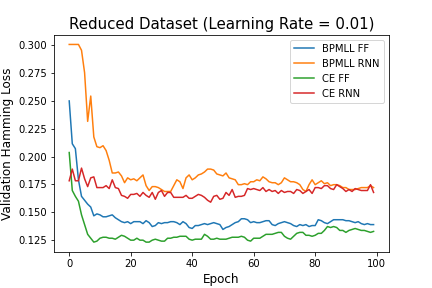
\includegraphics[width=0.32\textwidth,height=3cm]{Images/Reduced_Dataset_Learning_Rate_01.png}
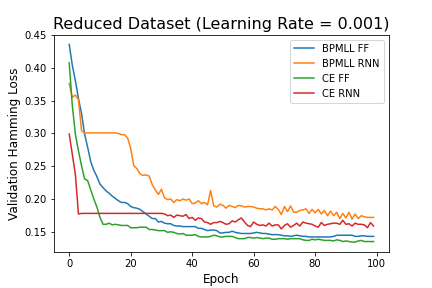
\includegraphics[width=0.32\textwidth,height=3cm]{Images/Reduced_Dataset_Learning_Rate_001.png}
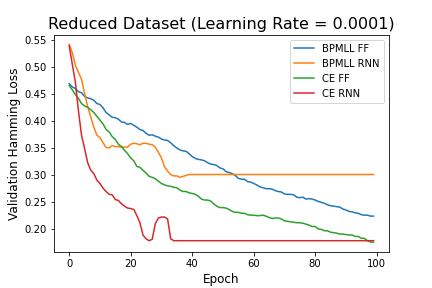
\includegraphics[width=0.32\textwidth,height=3cm]{Images/Reduced_Dataset_Learning_Rate_0001.png}        
\end{center}

\begin{center}

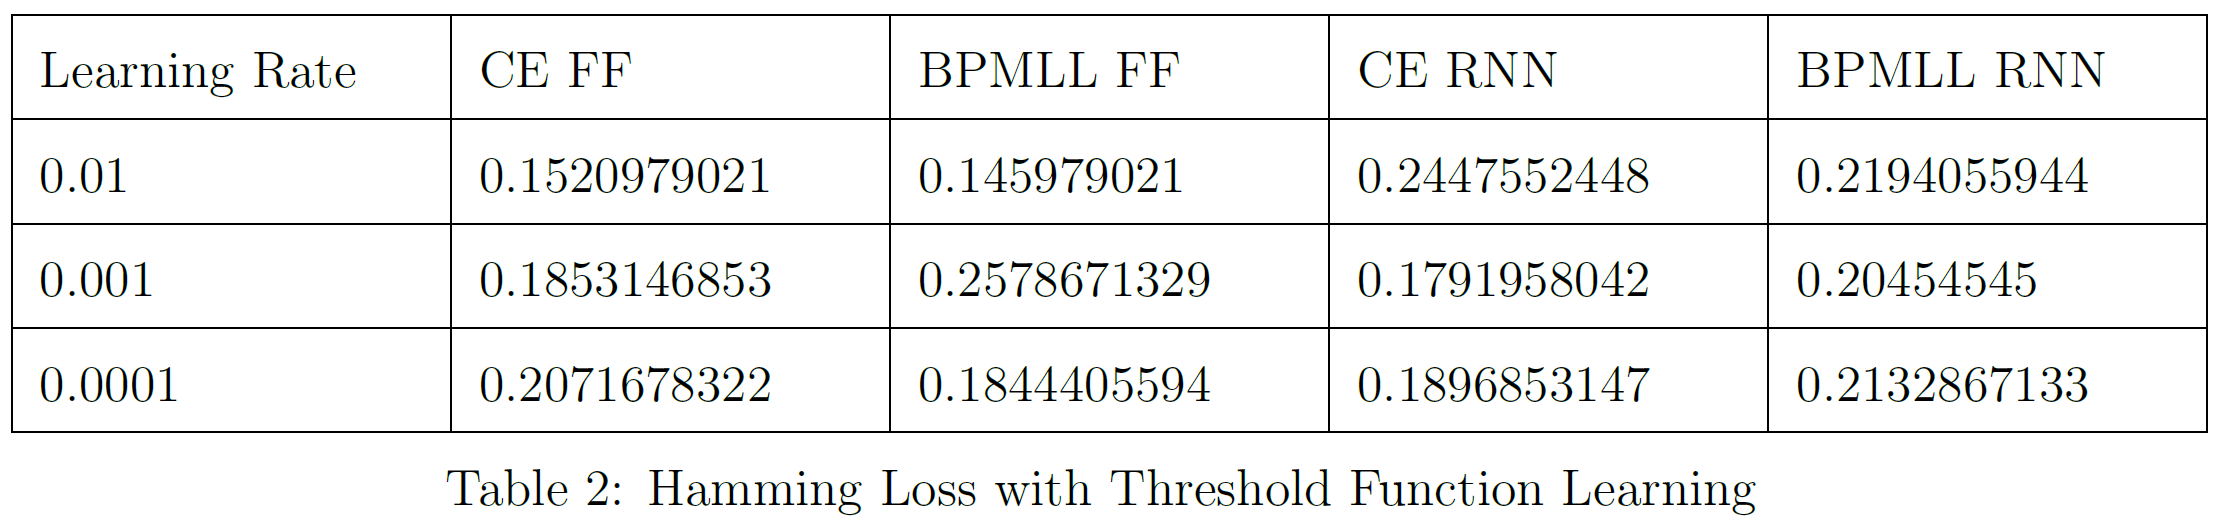
\includegraphics[width=1\textwidth,height=3cm]{Images/Threshold learning for reduced dataset.png}
\end{center}

Same conclusion for RNN and FF; BPMLL shows NO
better performance in hamming loss than cross entropy.
\end{frame}

\section{Discussion and Conclusions}

\begin{frame}[t]{Discussion and Conclusions: ANN Approaches}
    \vspace{-.2cm}
    \begin{enumerate}
        \footnotesize
        \only<2->{
        \item 
        The FF networks networks tend to outperform the RNNs.}
        
        \begin{itemize}
            \only<3->{
            \item[\rightarrow] 
            More parameters lead to overfitting in the bidirectional LSTM.}
            
            \only<4->{
            \item[\rightarrow]
            Single directinal LSTM can't escape locally optimal solution.}
            
            \only<5->{
            \item[\rightarrow]
            Training on more data may improve.}
        \end{itemize}
        
        \only<6->{
        \item
        The cross entropy networks tend to outperform the BPMLL networks.}
        
        \begin{itemize}
            \only<7->{
            \item[\rightarrow]
            The surface for the BPMLL loss with tanh activations has plateaus in which gradient descent can be very slow in comparison with the cross-entropy (\cite{bp_mll_revisited}). The case may be similar for ReLU activations.
            
            \begin{figure}[htp]
                \centering
                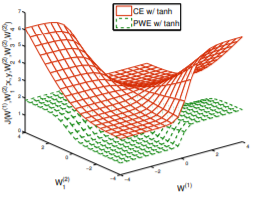
\includegraphics[width = 3.75cm]{Images/Nam_et_al_2014_bpmll_plateau.PNG}
            \end{figure}}
            
            \only<8->{
            \item[\rightarrow]
            While BPMLL is supposed to leverage correlations between labels, \cite{bp_mll_revisited} conjecture that these correlations also may cause overfitting.}
        \end{itemize}
    \end{enumerate}
\end{frame}

\begin{frame}[t]{Discussion and Conclusions: ANN Approaches (continued)}
    \begin{enumerate}
    \setcounter{enumi}{2}
    \only<1->{
        \item
        Models saw no improvement from using a learned threshold function.}
        
        \begin{itemize}
            \only<2->{
            \item[\rightarrow]
            Models could sufficiently separate predicted logits about $0.5$.}
            
            \only<3->{
            \item[\rightarrow]
            This approach may be more useful for models that require extensive resources for sufficient training (improved less extensively trained models).}
        \end{itemize}
    \end{enumerate}
\end{frame}

\begin{frame}[t]{References}
    \nocite{mlknn}
    \nocite{bpmll}
    \bibliography{mll_osu}
\end{frame}

\end{document}

